\documentclass[a4paper]{article}

%% Language and font encodings
\usepackage[english]{babel}
\usepackage[utf8x]{inputenc}
\usepackage[sfdefault,lf]{carlito}
%% The 'lf' option for lining figures
%% The 'sfdefault' option to make the base font sans serif
\usepackage[T1]{fontenc}
\renewcommand*\oldstylenums[1]{\carlitoOsF #1}
\usepackage{fancyhdr}
\setlength{\headheight}{41pt} 

%% Sets page size and margins
\usepackage[a4paper,top=3cm,bottom=2cm,left=3cm,right=3cm,marginparwidth=1.75cm]{geometry}

%% Useful packages
\usepackage{amsmath}
\usepackage{graphicx}
\usepackage[colorinlistoftodos]{todonotes}
\usepackage[colorlinks=true, allcolors=blue]{hyperref}
%\renewcommand{\headrulewidth}{0pt}
\fancyhead[L]{Posted: \today}
\fancyhead[R]{

\includegraphics[width=4cm]{engrXiv_banner.png}
}
\pagestyle{plain}
\title{Your Paper}
\author{A. Author}
\date{}

\begin{document}
\maketitle
\thispagestyle{fancy}

\begin{abstract}
Your abstract.
\end{abstract}

\section{Introduction}

Your introduction goes here! 

\section{Some examples to get started}

\subsection{How to include Figures}

First you have to make sure image file is located somewhere you can find it. If you are authoring on Overleaf, upload the image file from your computer using the upload link the project menu. Then use the includegraphics command to include it in your document. Use the figure environment and the caption command to add a number and a caption to your figure. See the code for Figure \ref{fig:frog} in this section for an example.

\begin{figure}
\centering
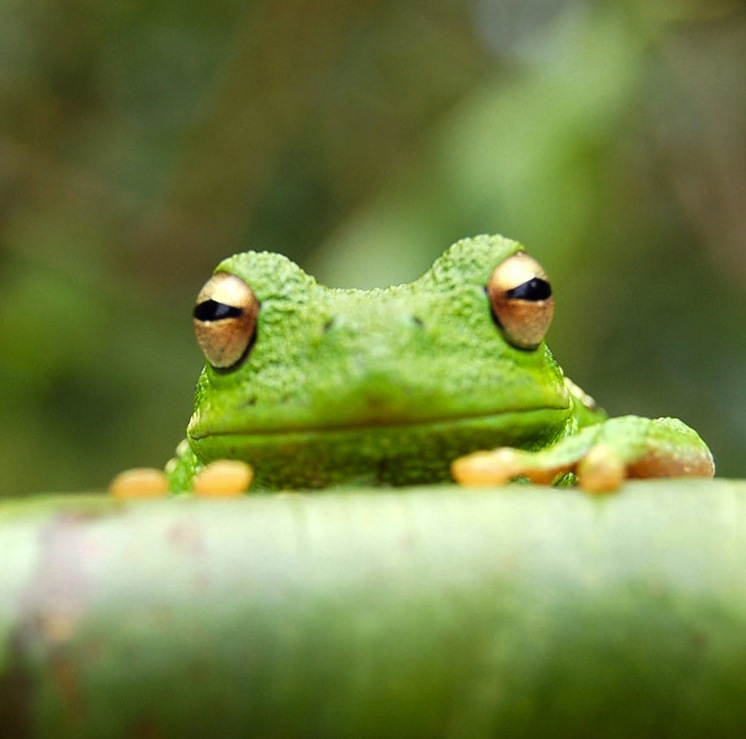
\includegraphics[width=0.3\textwidth]{frog.jpg}
\caption{\label{fig:frog}This is a frog.}
\end{figure}


\subsection{How to add Tables}

Use the table and tabular commands for basic tables --- see Table~\ref{tab:widgets}, for example. 

\begin{table}
\centering
\begin{tabular}{l|r}
Item & Quantity \\\hline
Widgets & 42 \\
Gadgets & 13
\end{tabular}
\caption{\label{tab:widgets}An example table.}
\end{table}

\subsection{How to write Mathematics}

\LaTeX{} is great at typesetting mathematics. Let $X_1, X_2, \ldots, X_n$ be a sequence of independent and identically distributed random variables with $\text{E}[X_i] = \mu$ and $\text{Var}[X_i] = \sigma^2 < \infty$, and let
\[S_n = \frac{X_1 + X_2 + \cdots + X_n}{n}
      = \frac{1}{n}\sum_{i}^{n} X_i\]
denote their mean. Then as $n$ approaches infinity, the random variables $\sqrt{n}(S_n - \mu)$ converge in distribution to a normal $\mathcal{N}(0, \sigma^2)$.


\subsection{How to create Sections and Subsections}

Use section and subsections to organize your document. Simply use the section and subsection buttons in the toolbar to create them, and we'll handle all the formatting and numbering automatically.

\subsection{How to add Lists}

You can make lists with automatic numbering \dots

\begin{enumerate}
\item Like this,
\item and like this.
\end{enumerate}
\dots or bullet points \dots
\begin{itemize}
\item Like this,
\item and like this.
\end{itemize}

\subsection{Inserting Citations}
Citations can be inserted using standard latex formatting by called the identifier in the .bib file. Like this \cite{einstein1935can}.

\bibliographystyle{apalike}
\bibliography{sample}

\end{document}
